\documentclass[accentcolor=tud1b,longdoc,nopartpage,table,oneside,bibtotoc, liststotoc,openright,colorbacktitle,inverttitle,numbersubsubsec,noresetcounter,11pt,noheadingspace,numbers=noenddot,article,parskip=half]{tudreport}

% Babel-Paket f. neue deutsche Rechtschreibung
\usepackage[ngerman]{babel}
\usepackage{graphicx}
% Eingabekodierung auf latin1 setzen
\usepackage[utf8]{inputenc}


% Font-Encoding auf T1 setzen
\usepackage[T1]{fontenc}
% footmisc behebt u.a. Probleme mit Fu�noten in Abschnittstiteln
\usepackage[stable]{footmisc}

% Einbinden von Grafiken erm�glichen
\usepackage{graphicx}

\usepackage{newunicodechar}
\newunicodechar{ß}{\ss}
% Paket xtab erm�glicht Umbrechen von langen Tabellen
\usepackage{xtab}

% picins erlaubt das Umflie�en von Abbildungen durch Text
% Untenstehendes renewcommand behebt den picins-bug, dass Abbildungen
% nicht im Abbildungsverzeichnis auftauchen
\usepackage{picins}
\makeatletter
\renewcommand\piccaption{\@dblarg{\@piccaption}}
\makeatother

\usepackage{verbatim}

% Einr�ckung bei Zeilenumbruch vermeiden
\setlength{\parindent}{0pt}
\setlength{\parskip}{9pt}
% Tiefe des Inhaltsverzeichnis (paragraphen werden mit aufgenommen)
\setcounter{secnumdepth}{4}
\setcounter{tocdepth}{4}
%Überschriften 
\addtokomafont{subsection}{\normalsize\bf}
\addtokomafont{subsubsection}{\normalsize\bf}
\addtokomafont{paragraph}{\small\bf}


%Silbentrennung von zusammengesetzten w�rtern
\usepackage[ngerman=ngerman-x-latest]{hyphsubst}
% Paket setspace erlaubt Umschalten auf 1.5fachen Zeilenabstand
\usepackage{setspace}


%%%%%%%%%%%%%%%%%%%%%%%%%%%%%%%%%%%%%%%%%%%%%%%%%%%%%%%%
%% Anpassungen von Literaturverzeichnis und Zitierweise%
\usepackage[hyphens]{url}
\usepackage[commabeforerest,authorformat=year,see,dotafter=bibentry,pages=format]{jurabib} % , ibidem=strict 
%\AddTo\bibsgerman{%
%\renewcommand*{\ibidemname}{ebd.}
%\renewcommand*{\ibidemmidname}{ebd.}
%}
%Trennzeichen zwischen Autoren im Zitat

%\AddTo\bibsgerman{%
%\def\jbpagename{S.}%
%\def\jbpagesname{S}%
%}

\renewcommand*{\jbbtasep}{ \& }
\renewcommand*{\jbbfsasep}{; }
\renewcommand*{\jbbstasep}{; }

%Trennzeichen zwischen Autoren im Literaturverzeichnis
\renewcommand*{\bibbtasep}{ \& }
\renewcommand*{\bibbfsasep}{; }
\renewcommand*{\bibbstasep}{ \& }

%Trennzeichen zwischen Herausgebern im Literaturverzeichnis
\renewcommand*{\bibbtesep}{; }
\renewcommand*{\bibbfsesep}{; }
\renewcommand*{\bibbstesep}{; }

%Unterdr�ckt, dass bei mehr als drei Autoren im Literaturverzeichnis
%mit "et al." abgek�rzt wird --> myjureco.bst-Datei wird zus�zlich ben�tigt!
\makeatletter
\def\jb@use@fullcite{%
\jbauthorfont{\jb@@author}\normalfont{\jbhowsepbeforetitle}\jb@@fulltitle}%
\makeatother

%In: erscheint vor dem Titel von Zeitschriften, Konferenzbeitr�gen, Sammelwerken
%und Herausgeberb�nden
%\AddTo\bibsall{\def\incollinname{\textbf{In:}}}
\renewcommand{\bibbtsep}{In: }
\renewcommand*{\bibjtsep}{In: }

%Vor- und Nachname des Herausgebers werden nicht fett gedruckt
\renewcommand*{\biblnfont}{} 
\renewcommand*{\bibfnfont}{}

%�ndert bei urldate das Pr�fix von "Zugriff am" zu "Abruf am"
\AddTo\bibsgerman{\renewcommand*{\urldatecomment}{Letzter Abruf: }}

%Setzt ein Komma zwischen der URL und "Abruf am"
\renewcommand*{\bibbudcsep}{, }

%Entfernt die Zeichen vor und nach der URL-Angabe im Literaturverzeichnis
\renewcommand*{\biburlprefix}{}
\renewcommand*{\biburlsuffix}{}

%Entfernt das Komma zwischen Jahrgang und Ausgabe
%und setzt die Ausgabe in Klammern
\renewcommand*\artnumberformat[1]{\unskip\space (#1)}

%Entfernt das Komma zwischen Adresse und Verlag
%und setzt daf�r ein Leerzeichen. Dies ist n�tig,
%da die Reihenfolge von Adresse und Verlag in myjureco vertauscht wird
%und kein Zeichen nach der Adresse erscheinen soll.
\renewcommand*\bpubaddr{}
\renewcommand*{\bibtfont}{\textit}
% Check if this gives errors
\renewcommand*{\bibapifont}{\textit}
\renewcommand*{\bibatsep}{,}
\renewcommand*{\ajtsep}{,}

%%%%%%%%%%%%%%%%%%%%%%%%%%%%%%%%%%%%%%%%%%%%%%%%%%%%%%%%


\usepackage{hyperref}
%Erm�glicht Hyperlinks zwischen Textstellen und zu externen Dokumenten
%% breaklinks=true/false: Gibt an, ob Links umgebrochen werden d�rfen.
%% linktocpage=true/false: im Inhaltsverzeichnis sind nur die Seitenzahlen
%% links, nicht der Text
%% colorlinks=true/false: Links werden eingef�rbt (Farben werden mit
%% linkcolor, anchorcolor \dots festgelegt)
%% linkcolor=Farbe: Farbe des verlinkten Textes, Dokument-interne Links
%% citecolor=Farbe: Farbe des verlinkten Textes, Links zum
%% Literaturverzeichnis
%% filecolor=Farbe: Farbe des verlinkten Textes, Links auf lokale Dateien
%% urlcolor=Farbe: Farbe des verlinkten Textes, externe URLs
%% frenchlinks=true/false: Links werden als smallcaps, anstatt farbig
%% dargestellt.
%% breaklinks=true/false: Gibt an, ob Links umgebrochen werden d�rfen.
\hypersetup{%
bookmarks=true,
unicode=false,
pdftoolbar=true,
pdfmenubar=true,
pdffitwindow=true,
pdfstartview={FitH}
  filecolor=black,
  breaklinks=true,
  colorlinks=true,
  citecolor=black,
  urlcolor=black,
  linkcolor=black,
  pdfpagemode=UseThumbs,
  pdftitle=Mustertitel,
  pdfauthor=Max Mustermann,
  pdfsubject=Musterthema,
  %pdfkeywords=xy
}




% Eigene Pakete hier 
\usepackage{rotating}
\usepackage{booktabs,dcolumn}
\usepackage{longtable}
\usepackage{paralist}
\usepackage{dcolumn}
\usepackage{nameref}
\usepackage[font=footnotesize ,font=bf]{caption}
\usepackage{subcaption}
%\usepackage{tex4ht}
\usepackage{listings}
\usepackage{etex}
\usepackage{tikz}
	\usetikzlibrary{patterns}
\usepackage{pgfplots}
%	\pgfplotsset{compat=1.11}
%	\usepgfplotslibrary{fillbetween}
\usepackage{icomma}
\usepackage{float}
\usepackage{amsmath}


\colorlet{punct}{red!60!black}
\definecolor{background}{HTML}{EEEEEE}
\definecolor{delim}{RGB}{20,105,176}
\colorlet{numb}{magenta!60!black}

\lstdefinelanguage{json}{
    basicstyle=\normalfont\ttfamily,
    numbers=left,
    numberstyle=\scriptsize,
    stepnumber=1,
    numbersep=8pt,
    showstringspaces=false,
    breaklines=true,
    frame=lines,
    backgroundcolor=\color{background},
    literate=
     *{0}{{{\color{numb}0}}}{1}
      {1}{{{\color{numb}1}}}{1}
      {2}{{{\color{numb}2}}}{1}
      {3}{{{\color{numb}3}}}{1}
      {4}{{{\color{numb}4}}}{1}
      {5}{{{\color{numb}5}}}{1}
      {6}{{{\color{numb}6}}}{1}
      {7}{{{\color{numb}7}}}{1}
      {8}{{{\color{numb}8}}}{1}
      {9}{{{\color{numb}9}}}{1}
      {:}{{{\color{punct}{:}}}}{1}
      {,}{{{\color{punct}{,}}}}{1}
      {\{}{{{\color{delim}{\{}}}}{1}
      {\}}{{{\color{delim}{\}}}}}{1}
      {[}{{{\color{delim}{[}}}}{1}
      {]}{{{\color{delim}{]}}}}{1},
}

% Anpassungen der R�nder an die Vorgaben des Lehrstuhls
% BACKUP \geometry{left=3cm, right=2cm, top=1.5cm, bottom=2cm}
\geometry{left=3cm, right=1.9cm, top=1.7cm, bottom=1.9cm,headsep=5mm, nomarginpar, includeall}

\hyphenation{In-for-ma-ti-on Apps}
%Zitationsstil: \citepara{Quelle} => (Quelle Jahreszahl)
\newcommand{\citepara}[1]{(\citealt{#1})}
%Zitationsstil: \pcite{Vgl.}{342}{Quelle} => (Vgl. Quelle, S. 342)
\newcommand*{\pcite}[3]{(\citealt[#1][#2]{#3})}
\newcommand{\citeparapage}[2]{(\citealt[#2]{#1})}
\newcommand{\citeflow}[1]{\citet{#1}}
%\newcommand{\citeflowpage}[2]{\citeauthor[#2]{#1}}

\newcommand*{\fullref}[1]{\hyperref[{#1}]{\autoref*{#1} \nameref*{#1}}}

\newcommand{\paragraphnoindent}[1]{\paragraph{#1}\noindent}

\usepackage{array}
\newcolumntype{L}[1]{>{\raggedright\let\newline\\\arraybackslash\hspace{0pt}}m{#1}}
\newcolumntype{C}[1]{>{\centering\let\newline\\\arraybackslash\hspace{0pt}}m{#1}}
\newcolumntype{R}[1]{>{\raggedleft\let\newline\\\arraybackslash\hspace{0pt}}m{#1}}

%Tabellenkonfig
\definecolor{lightgray}{gray}{0.9}
\let\oldtabular\tabular
\let\endoldtabular\endtabular
\renewenvironment{tabular}{\rowcolors{2}{white}{lightgray}\oldtabular}{\endoldtabular}
%Welche Ebenen bekommen die Linien des Desings in der Überschrift
\setcounter{seclinedepth}{1}

%Gepunktete Linien auch bei Verzeichnissen im Inhaltsverzeichnis
\usepackage{tocstyle}
\newtocstyle[KOMAlike][leaders]{alldotted}{}
\usetocstyle{alldotted}

%Kein Einzug in Verzeichnissen, Abbildung:/Tabelle: als Präfix vor Nummern            
\usepackage[titles]{tocloft}                                         
\setlength{\cftfigindent}{0cm}                                                     
\setlength{\cfttabindent}{0cm} 

\usepackage{tocstyle} 

\makeatletter 
\AfterTOCHead[lof]{% 
	\let\SAVEDNUMBERLINE\tocstyle@numberline 
	\renewcommand*{\tocstyle@numberline}[1]{% 
		\SAVEDNUMBERLINE{\figurename\ #1}% 
	}% 
} 
\AfterTOCHead[lot]{% 
	\let\SAVEDNUMBERLINE\tocstyle@numberline 
	\renewcommand*{\tocstyle@numberline}[1]{% 
		\SAVEDNUMBERLINE{\tablename\ #1}% 
	}% 
} 
\makeatother 

\renewcaptionname{ngerman}\figurename{Abbildung} 
\renewcaptionname{ngerman}\tablename{Tabelle}

\addtocontents{lof}{\protect\def\protect\autodot{: }}
\addtocontents{lot}{\protect\def\protect\autodot{: }}  

\bibliographystyle{jureco}
\title{Using Deep Learning Methods to Predict Tweet Engagement Metrics}

%\subtitle{Untertitel}

\subsubtitle{Masterarbeit
\linebreak Felix Peters | 1945834
\linebreak Master Wirschaftsinformatik}


\setinstitutionlogo[width]{images/is_logo.jpg}
%\referee{Gutachter 1}{Gutachter 2}








\begin{document}
\noindent
\setstretch{1.2}
\maketitle

\urlstyle{same}
\pagenumbering{roman}
%
%
%Die erste Seite der Arbeit mit Angaben zum Verfasser, zum Lehrstuhl und zum Thema
%
%
\vspace*{\fill}
\singlespacing 
\noindent Felix Peters \\
Matrikelnummer: 1945834 \\
Studiengang: Master Wirtschaftsinformatik \\\\
Masterarbeit \\
Thema: ``Using Deep Learning Methods to Predict Tweet Engagement Metrics'' \\\\
Eingereicht: 24. April 2018 \\\\
Betreuer: Prof. Dr. Peter Buxmann \\\\
Prof. Dr. Peter Buxmann \\
Fachgebiet Wirtschaftsinformatik | Software \& Digital Business \\
Fachbereich Rechts- und Wirtschaftswissenschaften \\
Technische Universität Darmstadt \\
Hochschulstraße 1 \\
64289 Darmstadt \\

\onehalfspacing

%\newpage
%\thispagestyle{empty}
\setcounter{page}{2}

%
%
%Ehrenwörtliche Erklärung
%
%

\section*{Ehrenwörtliche Erklärung gemäß \S 22 Abs. 7 APB der TU Darmstadt}
%\thispagestyle{empty}
Hiermit versichere ich, Felix Peters, die vorliegende Master-Thesis gemäß
\S 22 Abs. 7 APB der TU Darmstadt ohne Hilfe Dritter und nur mit den angegebenen
Quellen und Hilfsmitteln angefertigt zu haben. Alle Stellen, die Quellen
entnommen wurden, sind als solche kenntlich gemacht worden. Diese Arbeit hat in
gleicher oder ähnlicher Form noch keiner Prüfungsbehörde vorgelegen. \\
\\
Mir ist bekannt, dass im Falle eines Plagiats (\S 38 Abs. 2 APB) ein
Täuschungsversuch vorliegt, der dazu führt, dass die Arbeit mit 5,0 bewertet und
damit ein Prüfungsversuch verbraucht wird. Abschlussarbeiten dürfen nur einmal 
wiederholt werden. \\
\\
Bei der abgegebenen Thesis stimmen die schriftliche und die zur Archivierung
eingereichte elektronische Fassung gemäß \S 23 Abs. 7 APB überein. \\
\\
\\
\\
\noindent Darmstadt, den 24. April 2018
\\
\normalsize


%\newpage %Dieser Befehl muss hinzugefügt werden, falls man "twoside" anstatt "oneside" als Dokumentenoption benutzt
%\thispagestyle{empty} %Dieser Befehl muss hinzugefügt werden, falls man "twoside" anstatt "oneside" als Dokumentenoption benutzt


\pagestyle{headings}
        
\tableofcontents	
\newpage 
\listoffigures
\newpage
\listoftables
\clearpage

\setstretch{1.2}

\newcounter{seitenzahlroemisch}
\setcounter{seitenzahlroemisch}{\value{page}}

\pagenumbering{arabic}

\section{Einleitung}
\lbrack Zitat (optional)\rbrack :
\begin{quote}
\glqq Was ist die Absicht eines wissenschaftlichen Buches? Es stellt Gedanken dar und will den Leser von ihrer Gültigkeit überzeugen. Darüber hinaus will der Leser auch wissen: woher kommen diese Gedanken und wohin führen sie? Mit welchen Richtungen auf anderen Gebieten hängen sie zusammen?\grqq
\pcite{}{XVII}{carnap1974}
\end{quote}

Einer der wichtigsten Abschnitte der Arbeit ist die Einleitung, in der der Leser in das Thema eingeführt wird. Auch ein fachfremder Leser muss nach dem Lesen der Einleitung verstanden haben, warum das vorliegende Thema wichtig und erforschenswert ist. Die Einleitung sollte zum Weiterlesen animieren und das Interesse des Lesers wecken. Neben dieser Motivation der Arbeit sind die Zielsetzung und die Forschungsfragen der Arbeit zu konkretisieren. Diese werden im Laufe der Arbeit beantwortet. Abschließend folgt ein kurzer Überblick über die Arbeit.\par\medskip
In den folgenden Kapiteln wird ein typischer Aufbau einer wissenschaftlichen Arbeit dargestellt und jeweils anhand ihrer typischen Inhalte beschrieben. Dieser Aufbau ist jedoch nicht verbindlich und kann je nach Forschungsmethode stark variieren. Bitte klären Sie dies mit Ihrem jeweiligen Betreuer ab.\par\medskip
Nach der Einleitung (Kapitel 1) folgen die Grundlagen (Kapitel 2) und die Entwicklung eines Forschungsmodells (Kapitel 3). In Kapitel 4 wird die verwendete Forschungsmethode dargestellt und in Kapitel 5 die Forschungsergebnisse. Eine Diskussion der Ergebnisse findet in Kapitel 6 statt. Die Arbeit schließt mit einer abschließenden Zusammenfassung sowie mit einem Fazit und einem Ausblick (Kapitel 7).

%1
\section{Grundlagen}
Im Grundlagenkapitel stellen Sie das Basiswissen für die weiteren Kapitel vor. Hierzu können neben theoretischen Konzepten auch die historische Entwicklung und aktuelle Forschungsvorhaben gehören. Idealerweise bedient man sich hier mehrerer verschiedener Quellen, um die Ausführungen zu belegen.

Nachfolgend werden einige Formalitäten der Arbeit dargestellt.

Zur korrekten Verwendung der Vorlage benötigen Sie die TU Darmstadt Schriftart: \href{https://www.tu-darm-stadt.de/kommunikation_und_medien/corporate_design_1/schriften_und_vorlagen/index.en.jsp}{Schriften und Vorlagen der TU Darmstadt}
\subsection{Gliederungen}
Text
\subsubsection{Gliederungsebene 3}
Text
\paragraph{Gliederungsebene 4}
Text
\subsection{Aufzählungen}
\begin{itemize}
	\item Fehlende Motivation,
	\item Fehlende Agilität und 
	\item Fehlende Compliance.
\end{itemize}

Text 
\newpage
\subsection{Abbildungen}

\begin{figure}[h]
\begin{center}

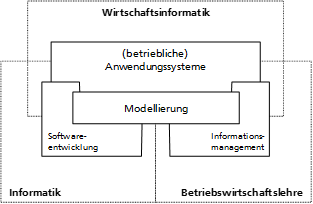
\includegraphics[width=10cm]{images/Abb2_3.png}
\caption{Einordnung der Wirtschaftsinformatik (angelehnt an Fink et al. 2001)}
\label{Abbildung2_3}
\end{center}
\end{figure}
Bitte achten Sie darauf, dass alle vorhandenen Abbildungen und Tabellen in einem inhaltlichen Zusammenhang mit dem Text stehen und Sie auf die entsprechende Abbildung (bspw. Abbildung 1) verweisen.
\subsection{Tabellen}
%hier Tabelle einfügen
\begin{table}[h]
\centering
\begin{tabular}{ccc}
\hline \textbf{Attribute} &\textbf{Typ}  & \textbf{1. Ausprägung (Beispiel)} \\ 
\hline Titel & \textit{STRING}& Aktiengesetz (AktG)  \\ 
Text& \textit{STRING} &  [Text des AktG]\\ 
Gültig von & \textit{DATE} & 01.01.2010 \\ 
Gültig bis & \textit{DATE} & - \\ 
Dok.-Besitzer & \textit{STRING} & Rechtsabteilung \\ 
Quelle & \textit{STRING}  & Deutsche Gesetze \\ 
Verplichtungsgrad & \textit{STRING} & verplichtend \\ 
\hline 
\end{tabular} 
\caption{Attribute der Anforderungsquellen im Metamodell}
\label{tab:tabelle 1}
\end{table}
\par\medskip

Tabelle 1 stellt eine beispielhafte Tabelle dar%2
\section{Entwicklung eines konzeptuellen Rahmens}
\label{cha:entwicklung}
Dieses Kapitel dient der Entwicklung eines konzeptuellen Rahmens auf Basis theoretischer Grundlagen, vorausgesetzt sie verfolgen einen positivistischen Ansatz. Hierfür leiten Sie Hypothesen aus verschiedenen sinnvoll kombinierten Quellen her. Hierdurch generieren Sie aus bestehendem Wissen neues Wissen, was eine Eigenleistung und somit ein wichtiger Bestandteil Ihrer Arbeit darstellt.

Sollte Ihre Arbeit nicht positivistisch ausgelegt sein, stellt dieser Abschnitt kein Pflichtkapitel der Arbeit dar. Alternativ beschreiben Sie Anforderungen für ein mögliches Konzept oder verzichten vollständig auf dieses Kapitel.

\textbf{Setzen Sie sich frühzeitig mit Ihrem Betreuer in Verbindung, um Ihre Gliederung abzustimmen und mögliche Missverständnisse zu beseitigen.}

Im Folgenden werden einige allgemeine Hinweise zu den Themen richtiges Zitieren und Literaturrecherche gegeben.


\subsection{Quellen und richtiges Zitieren}
Quellen können in Fußnote oder direkt im Text platziert werden. Alles was nicht Ihr eigenes Gedankengut darstellt, muss mit einer entsprechenden Quelle belegt werden. Hierbei können wörtliche und indirekte Zitate verwendet werden. Wörtliche Zitate sind immer mit der Seitennummer der Quelle anzugeben.

Beispiel für ein direktes Zitat:

\textit{\glqq The case study is a research strategy which focuses in understanding the dynamics present within single settings\grqq} \pcite{}{543}{eisenhardt1989}.

Beispiel für ein indirektes Zitat:

Eine explorative Fallstudie dient der Gewinnung von neuen Erkenntnissen und der Bildung von neuen Hypothesen über bestimmte Sachverhalte. Durch den Beitrag zum Theorieaufbau ist der Erkenntnisgewinn höher als bei einer reinen deskriptiven Fallstudie. In explorativen Fallstudien werden Phänomene in noch wenig erforschten Gebieten identifiziert und aus erkannten Zusammenhängen neue Hypothesen gebildet \citepara{eisenhardt1989}.

Alternativ kann die Quelle auch im  laufenden Text angegeben werden:

Nach \citeflow{eisenhardt1989} wird die Wichtigkeit der Fallauswahl oft unterschätzt. Die Fälle können zwar zufällig ausgewählt werden, dies ist aber weder notwendig noch wünschenswert.

Quellenangaben bestehen aus Autor, Jahr und ggf. Seitenangabe. Bei zwei Autoren sind beide Autoren zu nennen, bei mehreren Autoren nur der erste Autor mit dem Zusatz „et al.“.\newpage


\subsection{Zitieren mit Endnoten}
Im Rahmen der Erstellung von Arbeiten am Fachgebiet ISE ist das Literaturverwaltungsprogramm EndNote zu verwenden. Dieses steht auf der \href{http://www.ulb.tu-darmstadt.de/service/literaturverwaltung_start/endnote_ulb/endnote.de.jsp
}{ULB-Seite} zum Download verfügbar. 


\subsubsection{Lateinischer Text mit Zitaten für Erstellung des Literaturverzeichnisses}
\label{cha:source:latintext}
Lorem ipsum dolor sit amet, consectetur adipiscing elit. Sed vitae lacus eu augue semper lobortis vitae aliquet leo. Fusce eleifend sodales commodo \citepara{eisenhardt1989}. Mauris arcu metus, bibendum sagittis condimentum eget, placerat a enim \citepara{baechle2010}. Quisque sit amet sagittis lectus. Curabitur sit amet libero eu felis elementum mollis. Nullam odio diam, mollis vitae viverra ut, laoreet ut odio. Praesent facilisis suscipit consequat. Morbi feugiat rutrum erat, eu sagittis nibh rhoncus nec \citepara{melao2000}.

In euismod, arcu ut semper adipiscing, nibh odio ullamcorper arcu, ut scelerisque massa magna nec quam \citepara{benlian2013}. Curabitur bibendum nibh eget augue pellentesque iaculis \citepara{sheffi2005}. Praesent iaculis auctor gravida. Quisque congue, magna ut bibendum semper, enim tortor ultrices lorem, ac feugiat tortor lectus nec nunc \citepara{carnap1974}. Pellentesque habitant morbi tristique senectus et netus et malesuada fames ac turpis egestas. Lorem ipsum dolor sit amet, consectetur adipiscing elit. Fusce dignissim, augue a sodales tristique, neque dui mollis arcu, id interdum augue justo sed lacus \citepara{welchering2013}. Vestibulum ante ipsum primis in faucibus orci luctus et ultrices posuere cubilia Curae; Mauris euismod bibendum nulla, sed accumsan urna tempor sed. Etiam eget diam eros, sed aliquet dolor \citepara{broadbent1996}. Phasellus vitae quam in orci convallis pharetra. Donec sit amet imperdiet nisi \citepara{kayser2013}. Sed vel interdum orci. Praesent vulputate, dolor id varius egestas, enim libero cursus neque, a cursus sapien nulla ut augue. Nullam vitae tortor nisl, vitae cursus enim. Suspendisse eget metus ipsum, sit amet varius sem \citepara{shazly2013}.

\subsection{Literaturrecherche}
Anbei eine kurze Auflistung von möglichen Kanälen zur Literaturrecherche.

\textbf{Zu Verwaltung Ihrer Literatur benutzen Sie bitte das Programm EndNote, dieses wird kostenfrei von der TU zu Verfügung gestellt.}

\url{http://www.ulb.tu-darmstadt.de/angebot/service/literaturverwaltung/endnote.de.jsp}

\subsubsection{Angebot der ULB}
\begin{itemize}
\item Universitätsbibliotheken (\url{http://www.ulb.tu-darmstadt.de/})
\item Rechercheangebot der ULB (\url{http://www.ulb.tu-darmstadt.de/recherche/})
\end{itemize}

\subsubsection{Online-Datenbanken und -Bibliotheken}
\begin{itemize}
\item Elektronische Zeitschriftenbibliothek (EZB) \\
(\url{http://rzblx1.uni-regensburg.de/ezeit/fl.phtml?bibid=TUDA})
\item AIS Electronic Library (AISeL)\\
(\url{http://aisel.aisnet.org/})
\item Zeitschriftendatenbank (ZDB)\\
(\url{http://dispatch.opac.ddb.de/DB=1.1/srt=YOP/})
\item Datenbank-Infosystem (DBIS): Literatur- und Fakten-Datenbank\\
(\url{http://rzblx10.uni-regensburg.de/dbinfo/fachliste.php?bib_id=tud})
\item IEEE Xplore \\
(\url{http://ieeexplore.ieee.org/Xplore/dynhome.jsp?tag=1})
\item EBSCO: internationale wirtschafts-wiss. Zeitschriften\\ (\url{http://search.ebscohost.com})
\item Springer-Online: Bücher/Beiträge des Springer Verlags\\
(\url{http://www.springerlink.com})
\item WiSo Net: deutschsprachige Literatur zu Wirtschafts- und Sozialwissenschaften\\
(\url{www.wiso-net.de})

\end{itemize}

\subsubsection{Sonstiges}
\begin{itemize}
\item \textbf{Google Scholar:} Suchdienst für wissenschaftliche Recherchen (http://scholar.google.de)
\item \textbf{Verlagswebseiten} Recherche und den Zugriff auf Zeitschriften- und Zeitungsartikel und E-Books
\item \textbf{Webseiten von Unternehmen} für die Recherche von Unternehmensdaten und-statistiken sowie Unternehmensdatenbanken
\item \textbf{Webseiten von Bundes- und Landesbehörden sowie der EU}
 Statistisches Bundesamt (http://www.destatis.de)
\\Presse- und Informationsamt der Bundesregierung (http://www.bundesregierung.de)
\item \textbf{Webseiten von Marktforschungsinstituten}
(für Marktanteile und Verbraucheranalysen)
\item \textbf{Webseiten von Verbänden und Kammern}
Institut der deutschen Wirtschaft (http://www.deutsche-wirtschaft.de)
\end{itemize}%3
\section{Forschungsmethoden}
\label{cha:method}
In diesem Kapitel erläutern Sie ihre Forschungsmethode unter Verwendung von entsprechenden Quellen. Begründen Sie auch, warum Sie sich für diese Forschungsmethode entschieden haben und warum sie geeignet ist, die vorliegende Forschungsfrage zu beantworten.%4
\section{Forschungsergebnisse}
\label{cha:result}
In Kapitel „Forschungsergebnisse“ stellen Sie die Ergebnisse ihrer Arbeit dar. An dieser Stelle nehmen Sie noch keine Interpretation oder Erläuterung der Ergebnisse vor, sondern beschreiben rein deskriptiv ihre Befunde. Eine Auswertung findet im nachfolgenden Kapitel statt.%5
\section{Diskussion}
\label{cha:diskussion}
Im vorletzten Abschnitt diskutieren Sie Ihre Ergebnisse und stellen den Beitrag für die Praxis und für die Forschung dar. Gehen Sie auch auf die Einschränkungen Ihrer Arbeit ein.%6
%\addtocontents{toc}{\protect\newpage}
\section{Zusammenfassung und Ausblick}
\label{cha:fazit}
% Wohin sind wir gekommen
Zuletzt fassen Sie Ihre Arbeit kurz zusammen und stellen Ihre wichtigsten Schritte, Ergebnisse und Befunde dar. Geben Sie auch einen Ausblick auf mögliche anknüpfende Forschungsarbeiten. Außerdem findet sich hier Platz für eine kritische Hinterfragung einzelner Teilaspekte und auch für Ihre eigene Meinung.

\subsection{Abgabedokument}
% Was wurde in der Arbeit alles gemacht
% Roten Faden aufgreifen
% TODO Pr�sens oder Pr�teritum
\textbf{Abschlussarbeiten} (Bachelor-, Master-, Diplomarbeit) sind in zweifacher Ausführung, ein-seitig bedruckt und gebunden abzugeben. Dazu auf CD die Abschlussarbeit in digitaler Form (z.B. Word und PDF), inkl. der Endnote-Projektdatei und der Grafiken. \par\medskip
Für \textbf{Seminar- und Studienarbeiten} genügt eine ungebundene einfache Ausführung, ebenfalls einseitig bedruckt. Die Seminar-/Studienarbeit in digitaler Form inkl. der Endnote Projektdatei sind zusätzlich per E-Mail einzureichen.

\pagenumbering{Roman}
\bibliography{bibliography/referenzen}

%
%
%
%Appendix
%
%

\appendix

\section{Appendix}
\label{ch:appendix}

\subsection{User groups}
\label{sec:user_groups}

A detailed list of all examined Twitter accounts is omitted here for the sake
of brevity.
User groups were assembled as Twitter lists in the author's profile.
Find links to all lists in the following:

\begin{enumerate}
\item Celebrity user group: \url{https://twitter.com/_fpeters/lists/celebrities}
\item Politician user group: \url{https://twitter.com/_fpeters/lists/us-politicians}
\item Company user group: \url{https://twitter.com/_fpeters/lists/fortune-500}
\end{enumerate}

\subsection{Confusion matrices}
\label{sec:confusion_matrices}

Confusion matrices for favorite classification were omitted in the results chapter.
They are displayed in the following.

\begin{figure}[h]
\begin{subfigure}{.4\textwidth}
  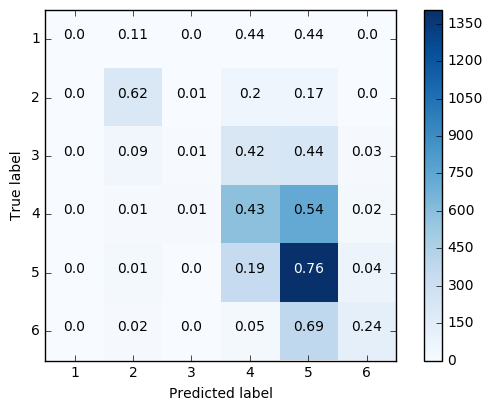
\includegraphics[width=.95\linewidth]{img/celeb_lin_cm_favorites}
  \caption{Celebrity data set}
  \label{fig:lin_fav_distr_sub1}
\end{subfigure}%
\begin{subfigure}{.4\textwidth}
  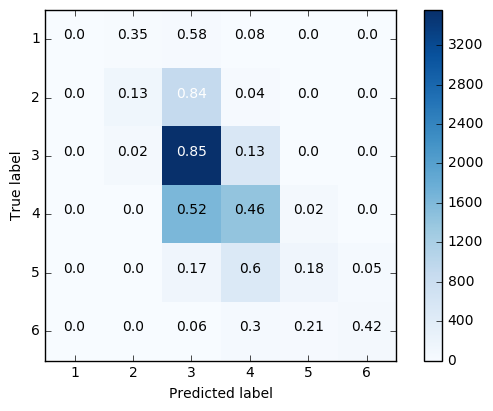
\includegraphics[width=.95\linewidth]{img/polit_lin_cm_favorites}
  \caption{Politician data set}
  \label{fig:lin_fav_distr_sub2}
\end{subfigure}
\begin{subfigure}{.4\textwidth}
  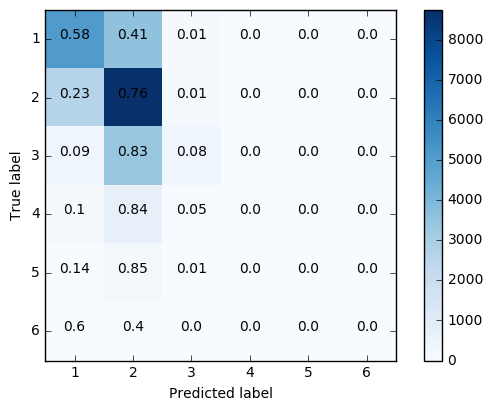
\includegraphics[width=.95\linewidth]{img/corp_lin_cm_favorites}
  \caption{Company data set}
  \label{fig:lin_fav_distr_sub3}
\end{subfigure}%
\begin{subfigure}{.4\textwidth}
  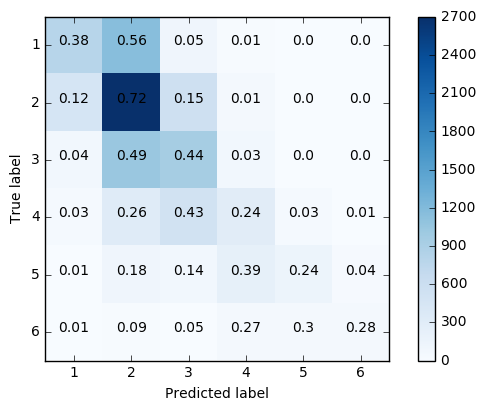
\includegraphics[width=.95\linewidth]{img/comb_lin_cm_favorites}
  \caption{Combined data set}
  \label{fig:lin_fav_distr_sub3}
\end{subfigure}%
\caption{Confusion matrices for linear retweet classification models}
\label{fig:lin_fav_cm}
\end{figure}

\begin{figure}[h]
\begin{subfigure}{.4\textwidth}
  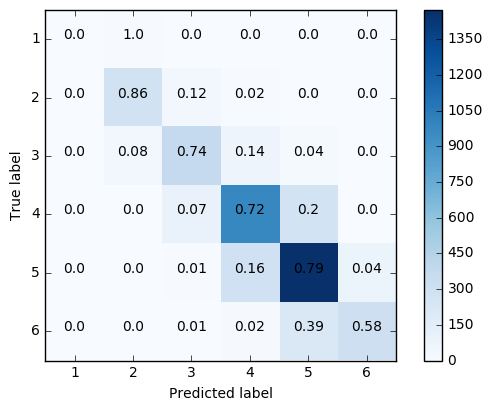
\includegraphics[width=.95\linewidth]{img/celeb_d1_cm_favorites}
  \caption{Celebrity data set}
  \label{fig:d1_fav_distr_sub1}
\end{subfigure}%
\begin{subfigure}{.4\textwidth}
  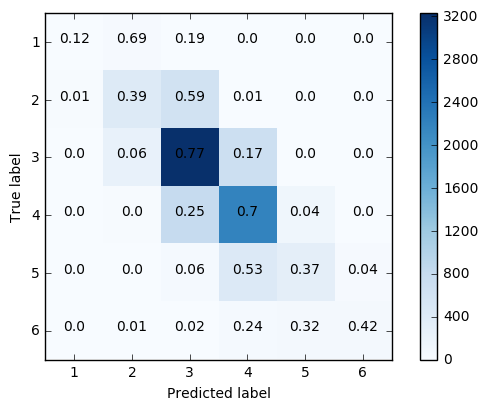
\includegraphics[width=.95\linewidth]{img/polit_d1_cm_favorites}
  \caption{Politician data set}
  \label{fig:d1_fav_distr_sub2}
\end{subfigure}
\begin{subfigure}{.4\textwidth}
  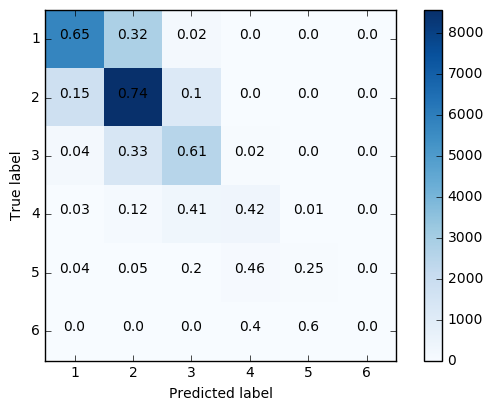
\includegraphics[width=.95\linewidth]{img/corp_d1_cm_favorites}
  \caption{Company data set}
  \label{fig:d1_fav_distr_sub3}
\end{subfigure}%
\begin{subfigure}{.4\textwidth}
  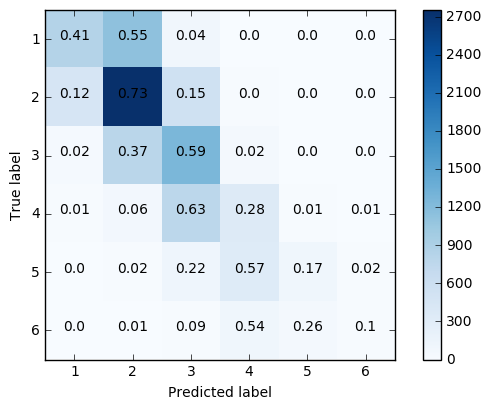
\includegraphics[width=.95\linewidth]{img/comb_d1_cm_favorites}
  \caption{Combined data set}
  \label{fig:d1_fav_distr_sub4}
\end{subfigure}%
\caption{Confusion matrices for deep feedforward classification models}
\label{fig:d1_fav_cm}
\end{figure}

\begin{figure}[h]
\begin{subfigure}{.4\textwidth}
  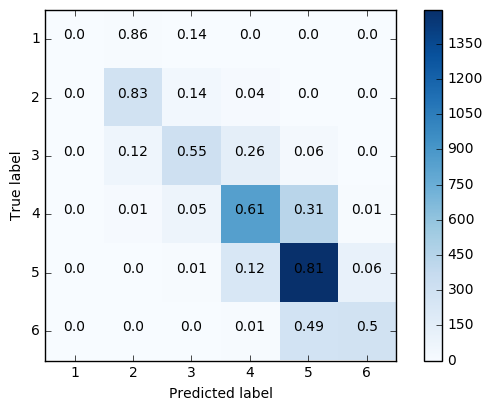
\includegraphics[width=.95\linewidth]{img/celeb_d2_cm_favorites}
  \caption{Celebrity data set}
  \label{fig:d2_fav_distr_sub1}
\end{subfigure}%
\begin{subfigure}{.4\textwidth}
  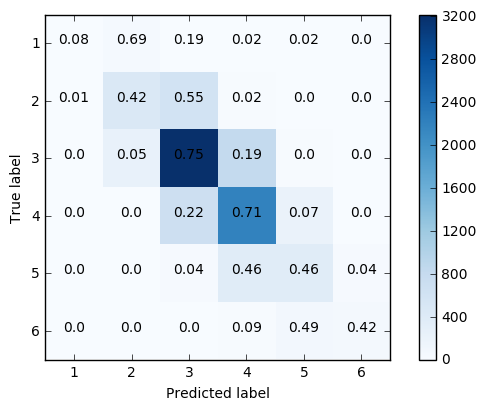
\includegraphics[width=.95\linewidth]{img/polit_d2_cm_favorites}
  \caption{Politician data set}
  \label{fig:d2_fav_distr_sub2}
\end{subfigure}
\begin{subfigure}{.4\textwidth}
  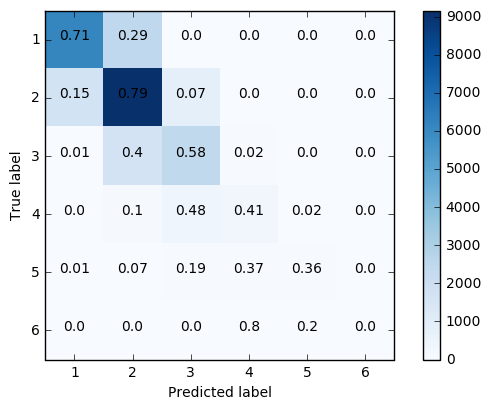
\includegraphics[width=.95\linewidth]{img/corp_d2_cm_favorites}
  \caption{Company data set}
  \label{fig:d2_fav_distr_sub3}
\end{subfigure}%
\begin{subfigure}{.4\textwidth}
  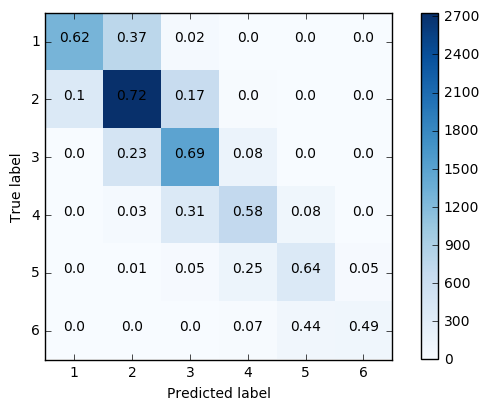
\includegraphics[width=.95\linewidth]{img/comb_d2_cm_favorites}
  \caption{Combined data set}
  \label{fig:d2_fav_distr_sub4}
\end{subfigure}%
\caption{Confusion matrices for multi-input deep neural networks}
\label{fig:d2_fav_cm}
\end{figure}


\end{document}

